\documentclass[10pt,a4paper]{book}
\usepackage{amsmath}
\usepackage{amsfonts}
\usepackage{amssymb}
\usepackage[english]{babel}
\usepackage{float}
\usepackage[left=2cm,right=2cm,top=2cm,bottom=2cm]{geometry}
\usepackage{graphicx}
\usepackage{hyperref} % Used for external links
\usepackage[utf8]{inputenc}
\usepackage{listings} % Used for source code listing
\usepackage{mathtools}

\setcounter{tocdepth}{3}

% Source code listing's parameters
\lstset{
  frame=single,
  keepspaces=true,
%  title=\lstname
}

\title{Third SPICE Exercise\\{\small{Fundamentals Of Electronics - a.a. 2018-2019 -
University of Padua (Italy)}}}
\author{Pietro Prandini (mat. 1097752)}

\begin{document}
\maketitle

\vspace*{\fill}
% License
\begin{center}
\tiny{This work is licensed under the Creative Commons Attribution-ShareAlike 4.0 International License. To view a copy of this license, visit \href{http://creativecommons.org/licenses/by-sa/4.0/}{http://creativecommons.org/licenses/by-sa/4.0/} or send a letter to Creative Commons, PO Box 1866, Mountain View, CA 94042, USA.}
\end{center}

\tableofcontents

\chapter{Differential amplifier with MOS current source}

\begin{figure}[h]
  \centering
  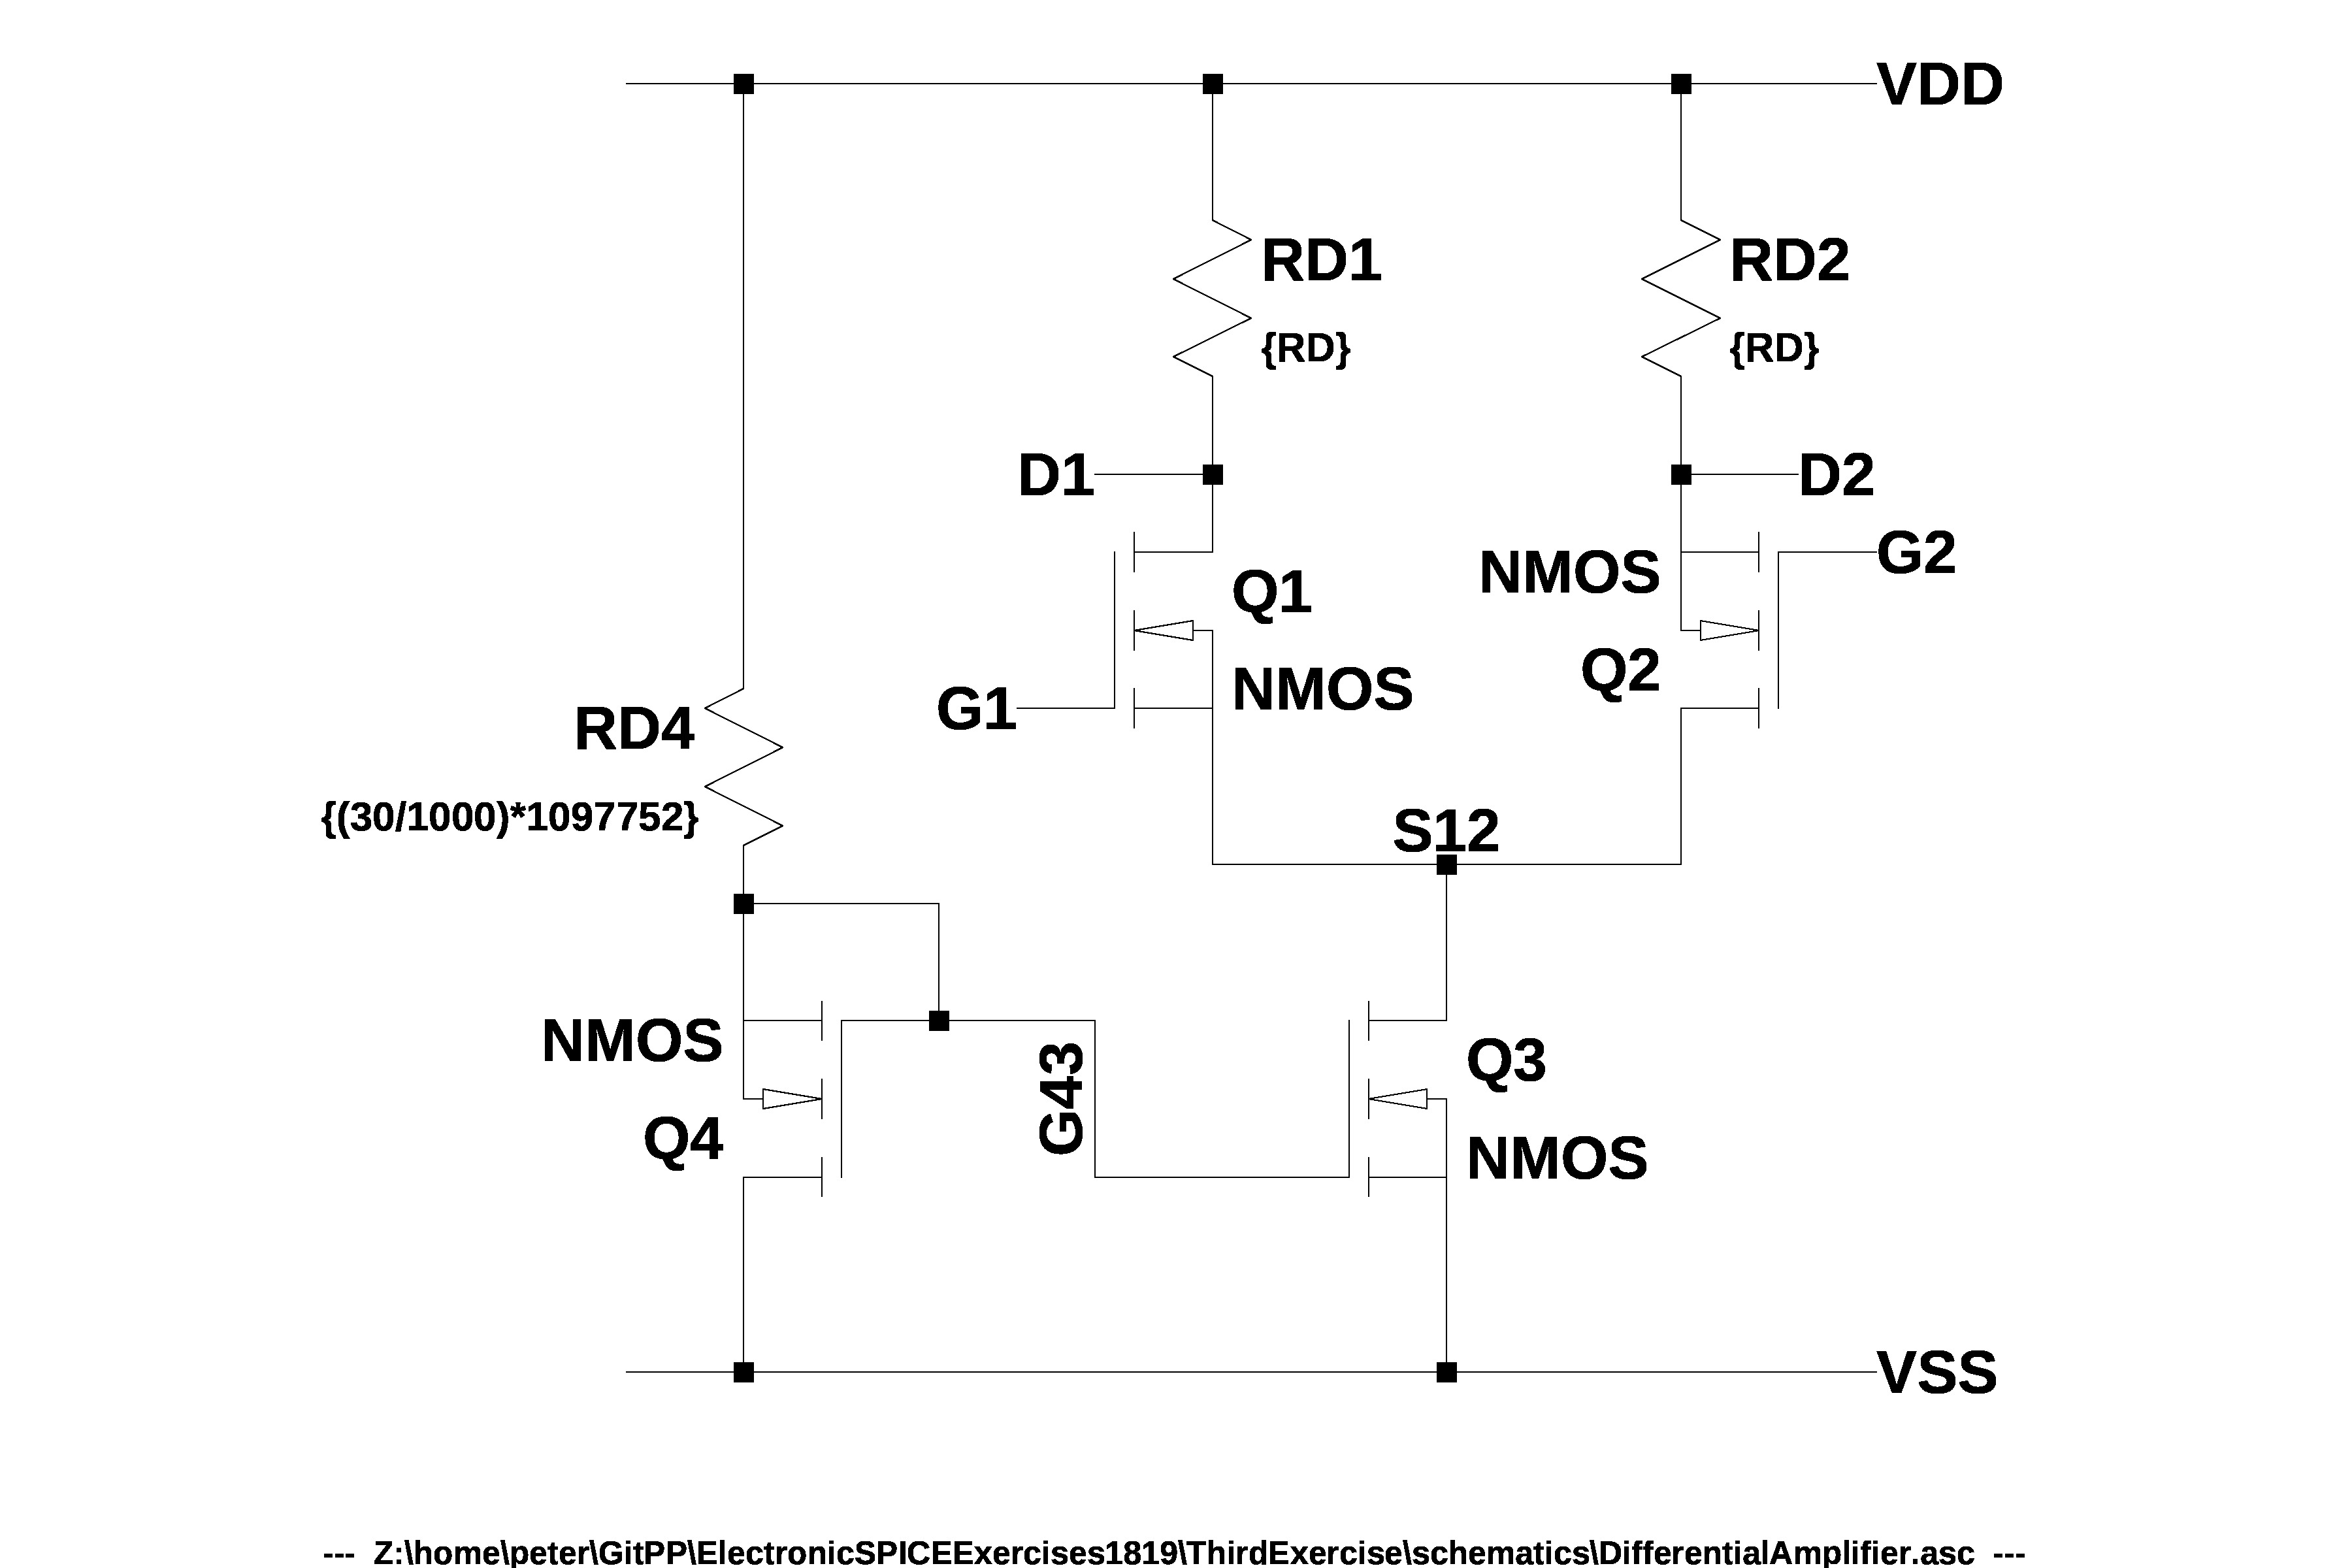
\includegraphics[width=12cm]{schematics/DifferentialAmplifier.jpg}
  \caption{Differential amplifier with MOS current source}
  \label{DifferentialAmplifier}
\end{figure}

\section{SPICE Operating Point analysis}
\lstinputlisting{netlist/DifferentialAmplifier.cir}
\lstinputlisting{netlist/DifferentialAmplifier.op}

\end{document}
